L'utilisation de métaux par les technologies bas-carbone s'intensifie dans les scénarios ambitieux de décarbonation. Les principales technologies responsables de cette intensification sont les réseaux électriques d'une part et les véhicules électriques d'autre part. Comme exposé en figure \ref{fig:metals_demand} la consommation en cobalt pour la fabrication des batteries des véhicules électriques pourrait dépasser la consommation mondiale pour tout les usages de cobalt en 2021.\smallbreak
L'aval de ces matières brutes - illustré en figure \ref{fig:supply_key_elements} - est constitué de deux étapes capitales pour l'approvisionnement : le raffinage et la fabrication des composants intermédiaire.\smallbreak
L'étape de raffinage est actuellement dominée par l'industrie chinoise dans l'ensemble des métaux critiques pour la décarbonation (voir fiches métaux section \ref{section:approvisionnement}). De manière générale, chaque métal possède au moins un type de chaîne d'approvisionnement pour le raffinage. Mais les métaux peuvent avoir plusieurs filières de raffinage en raison de la diversité de leur état au moment d'extraction. Par exemple, le nickel issu de minerai d'oxyde est particulièrement difficile à convertir en nickel de classe 1 (très pur) contrairement à du nickel issu de minerai de sulfure (\cite{iea_role_2021}).\smallbreak
La Chine possède aussi une place très dominante dans la fabrication des composants, voire sur la fabrication finale de la technologie. L'étape de fabrication des composants peut se décomposer en plusieurs sous-étapes. La fabrication des batteries est précédée de celle de l'anode et de la cathode. Cette dernière concentre la majorité des enjeux d'approvisionnement (voir figure \ref{fig:EV_key_elements}). Les chaînes d'approvisionnement autour des installations photovoltaïques et éoliennes contiennent également plusieurs maillons comme présenté en figure \ref{fig:electricity_key_elements}.\smallbreak
Même si l'explosion de la demande en véhicules électriques et en installations photovoltaïques et éoliennes offre la possibilité à d'autres pays de saisir la croissance des marchés, les projets industriels en développement placent progressivement l'industrie chinoise dans une position encore plus prépondérante. L'industrie chinoise pourrait être en mesure de satisfaire la demande en modules photovoltaïques dans les scénarios les plus ambitieux de décarbonation jusqu'en 2030 (\cite{iea_energy_2023}).\smallbreak
Il convient de noter que certains maillons du déploiement de technologies bas-carbone sont moins soumis aux risques géopolitiques : l'étude et le développement, l'installation et l'exploitation d'infrastructures. Néanmoins, il n'est pas garanti que la valeur ajoutée de ces maillons soit essentiellement locale. (voir encadré \hyperref[VAENR]{\textit{Répartition de la VA sur le PV et l'éolien en France}})
\begin{figure}[!b]
    \centering
    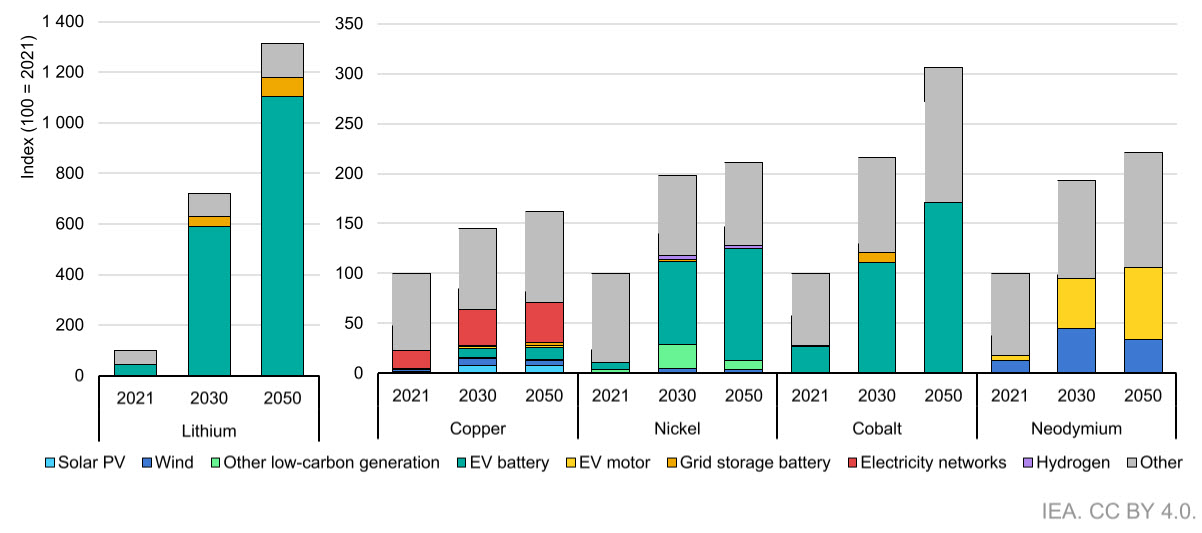
\includegraphics[width=\textwidth]{Images/supply_chain/metals_demand.jpg}
    \caption{Evolution de la demande en métaux dans lans le scénario NZE de l'AIE (\cite{iea_energy_2023})}
    \label{fig:metals_demand}
\end{figure}

\begin{figure}[!t]
\centering
\begin{subfigure}{0.9\textwidth}
    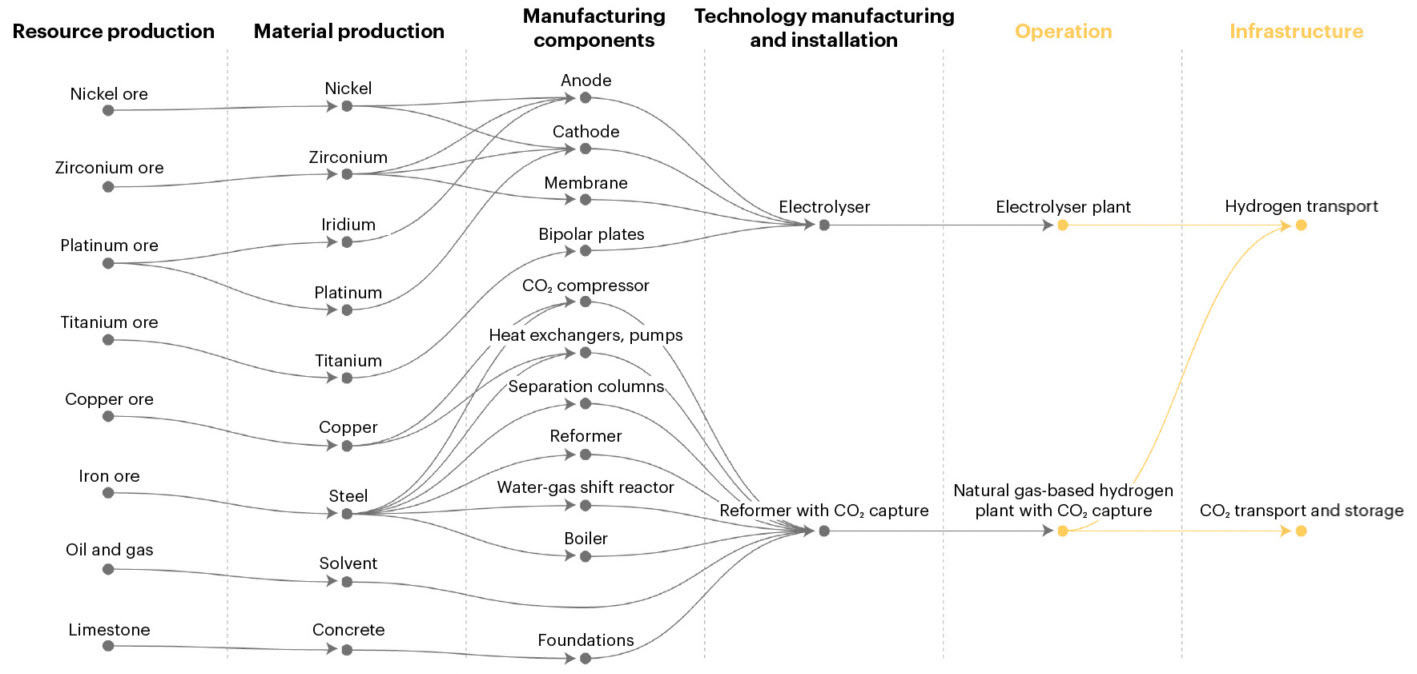
\includegraphics[width=\textwidth]{Images/supply_chain/key_elements_h2.jpg}
    \caption{Hydrogène bas-carbone}
    \label{fig:h2_key_elements}
\end{subfigure}
\hfill
\begin{subfigure}{0.9\textwidth}
    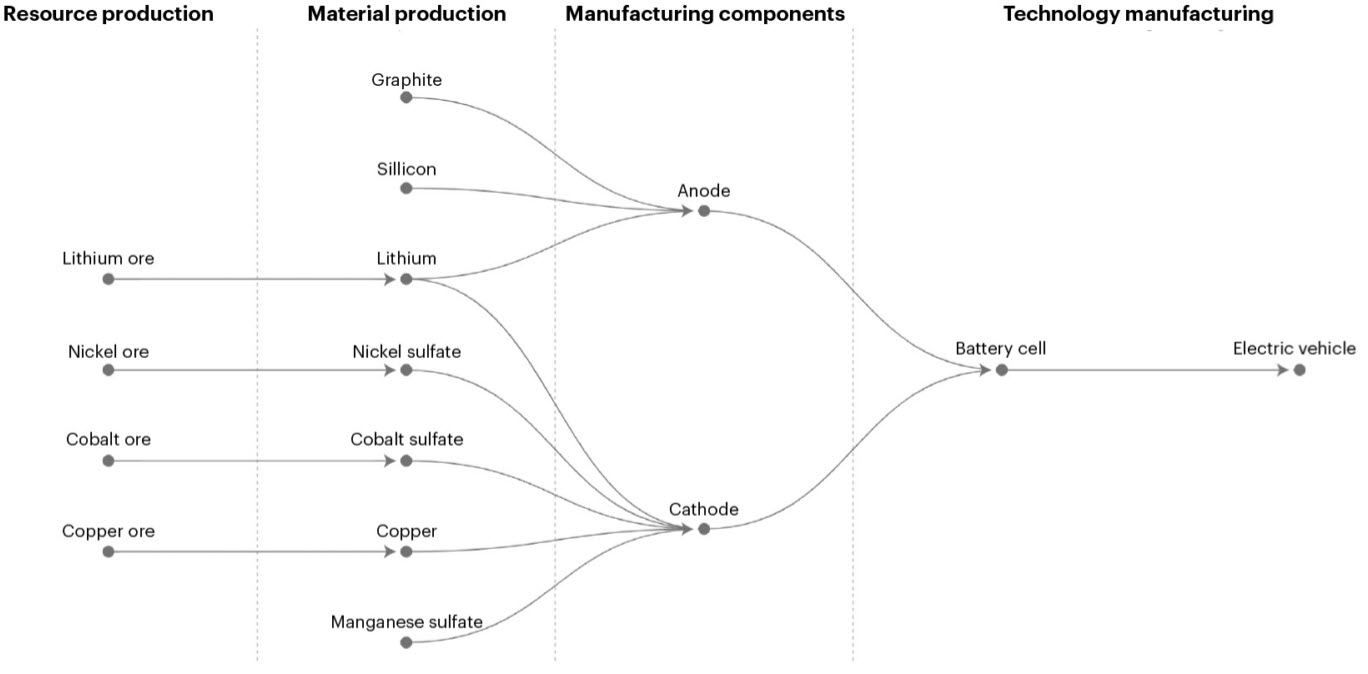
\includegraphics[width=\textwidth]{Images/supply_chain/key_elements_VE.jpg}
    \caption{Véhicules électriques}
    \label{fig:EV_key_elements}
\end{subfigure}
\hfill
\begin{subfigure}{0.9\textwidth}
    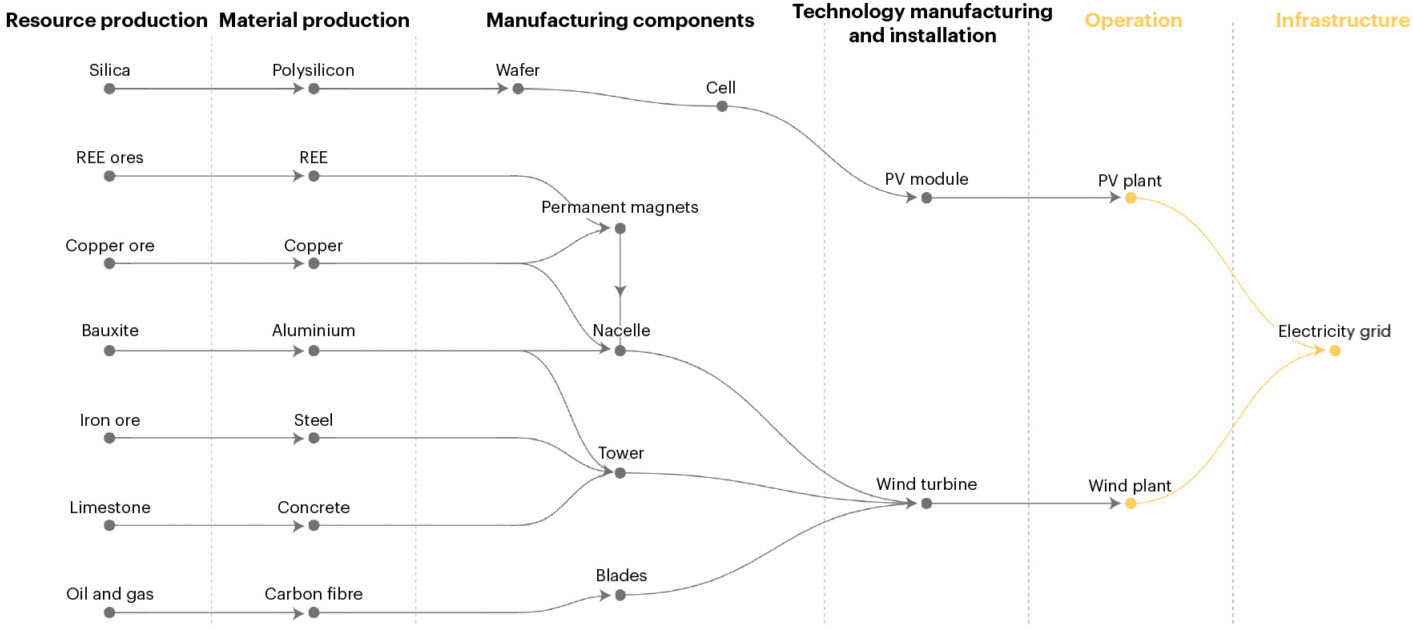
\includegraphics[width=\textwidth]{Images/supply_chain/key_elements_electricity.jpg}
    \caption{Electricité bas-carbone}
    \label{fig:electricity_key_elements}
\end{subfigure}  
\caption{Eléments clés des chaînes d'approvisonnements des technologies bas-carbone (\cite{iea_energy_2023})\\}
\label{fig:supply_key_elements}
\end{figure}
\clearpage
\begin{center}
    \boxput*(0,1){
        \colorbox{white}{Répartition de la valeur ajoutée sur le photovoltaïque et l'éolien en France}
    }{
    \setlength{\fboxsep}{15pt}
    \fbox{\begin{minipage}{14cm} 
    
    \begin{center}
        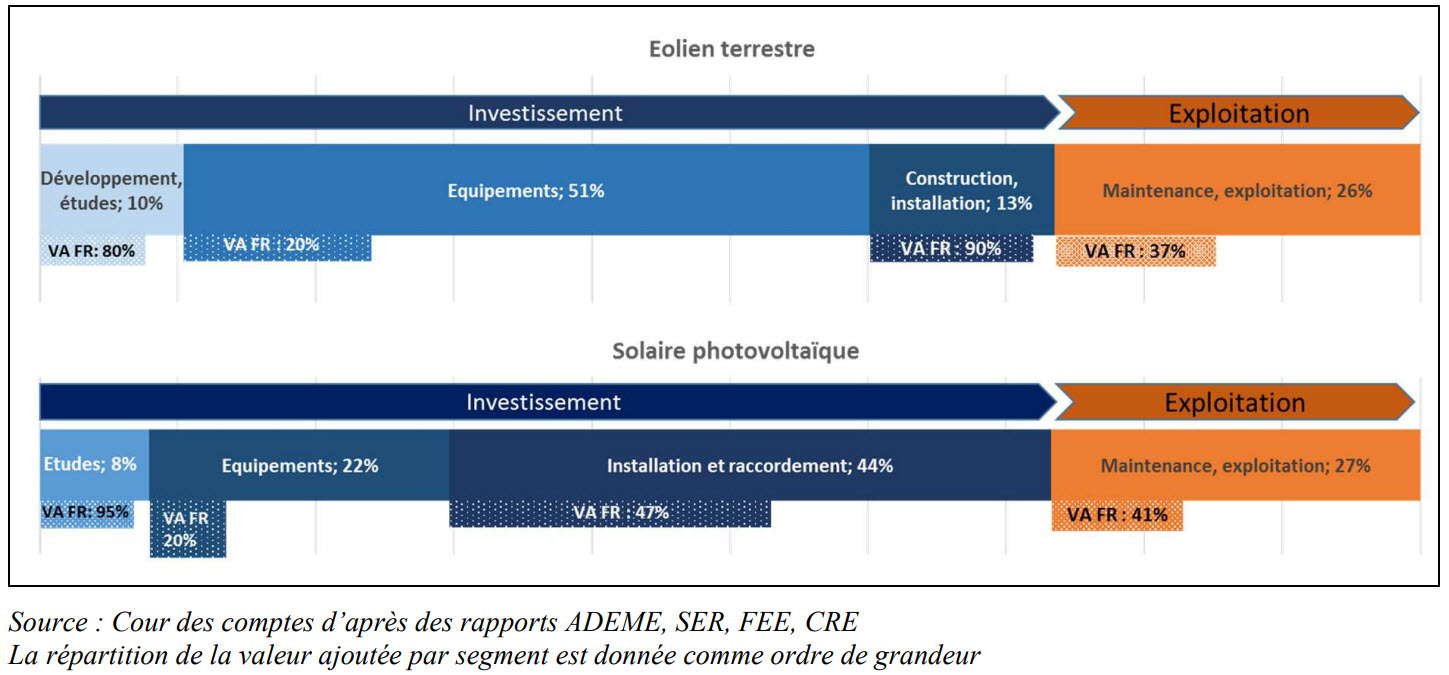
\includegraphics[width=\textwidth]{Images/supply_chain/VA_eolien_PV_cour.jpg}
\end{center}
    
Dans le domaine des énergies renouvelables, la chaîne de valeur comprend un grand nombre d'activités différentes. Ces activités incluent les études et l'ingénierie en amont, la fabrication de matériel et d'équipements, la construction et l'installation, l'exploitation et la maintenance, et enfin le démantèlement et le recyclage en aval.\smallbreak
Par exemple, dans le secteur du solaire, la France dispose de deux entreprises de fabrication intégrée de module photovoltaïque. Photowatt fait partie du groupe EDF et maîtrise l'ensemble de la fabrication des modules photovoltaïques, de la fabrication du lingot à partir de silicium jusqu'au recyclage (à 96\%). SunPower fait partie du Groupe TotalEnergies. La capacité de production reste néanmoins faible par rapport au marché français : environ 200 MWc par an pour Photowatt et moins de 100 MWc par an pour SunPower.\smallbreak
La France ne dispose pas d'ensemblier d'éolien terrestre et a perdu ses champions sur l'éolien en mer. Après s’être lancé en 2007 dans l’éolien en mer, Areva a cédé, en septembre 2016, ses activités à l’entreprise Gamesa, son partenaire espagnol dans la co-société Adwen. Le modèle de turbine Siemens sera fabriqué dans les deux futures usines construites au Havre. L’usine de fabrication d’éoliennes de Saint-Nazaire d’Alstom, a quant à elle été reprise par General Electric fin 2015.\smallbreak
De manière générale, il a été évalué qu'en France 40\% de la chaîne de valeur de l'éolien et du photovoltaïque est française. D'après le président directeur-général d'EDF, une chaîne de valeur 100\% française de l'éolien et du PV implique une hausse des coûts de l'ordre de 20\%.
\\[0.5cm]
\textit{Sources : \cite{cour_des_comptes_soutien_2018},\cite{photowatt_photowatt_2022},\cite{totalenergies_energie_2012},\cite{noauthor_souverainete_2023}}

    \end{minipage}}
    }
\end{center}
\label{VAENR}
~\\
\textbf{Photovoltaïque}
\smallbreak
La Chine est de loin le plus grand fournisseur de composants dans chaque étape de la chaîne d'approvisionnement du photovoltaïque avec une capacité de production de 340 GW/an (voir figure \ref{fig:PV_sankey}). Cela est dû à des coûts de production très faibles en Chine (voir figure \ref{fig:PV_cost}). L'écart des coûts de production entre l'Europe et la Chine se joue sur plusieurs facteurs : le coût de l'énergie, le coût de la main d'oeuvre et le coût de la dépréciation. Si ce dernier est plus faible en Chine, c'est en grande partie dû au coût du capital plus faible dans ce secteur et à la grande taille des unités de production.\smallbreak
Bien qu'ayant permis une importante chute des prix du photovoltaïque, la domination chinoise place les pays européens ambitieux quant au développement de cette technologie dans une situation de dépendance. Une sortie de cette dernière imposerait aux pays européens un coût d'investissement d'environ 500 M€ par GW de production photovoltaïque intégré (voir figure \ref{fig:PV_investment}).

\begin{figure}[!t]
\centering
\begin{subfigure}{0.8\textwidth}
    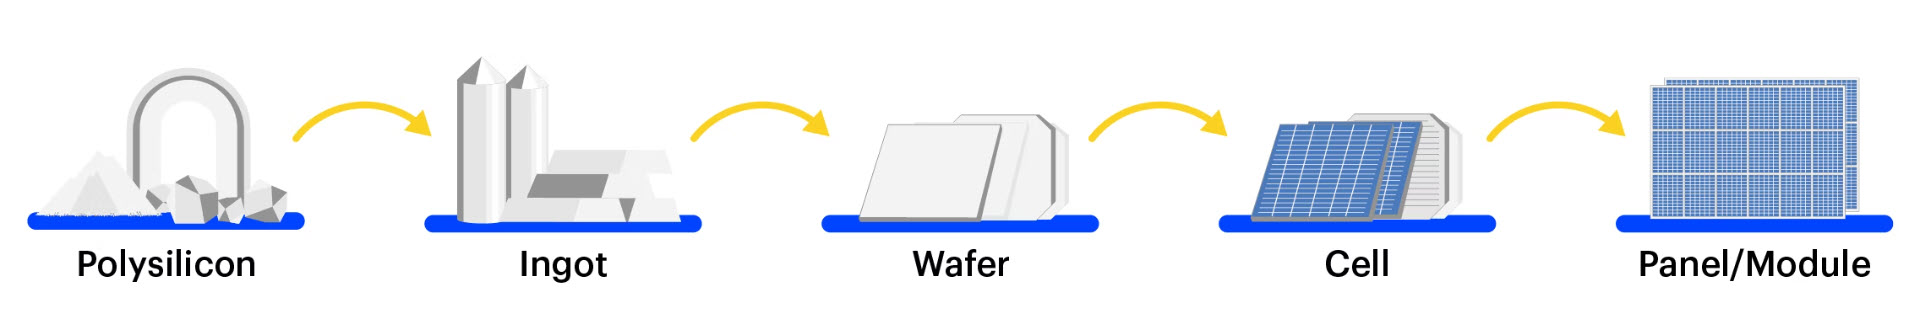
\includegraphics[width=\textwidth]{Images/supply_chain/PV_supply_chain.jpg}
    \caption{Etapes de fabrication d'un module photovoltaïque}
    \label{fig:PV_supply}
\end{subfigure}
\hfill
\begin{subfigure}{0.8\textwidth}
    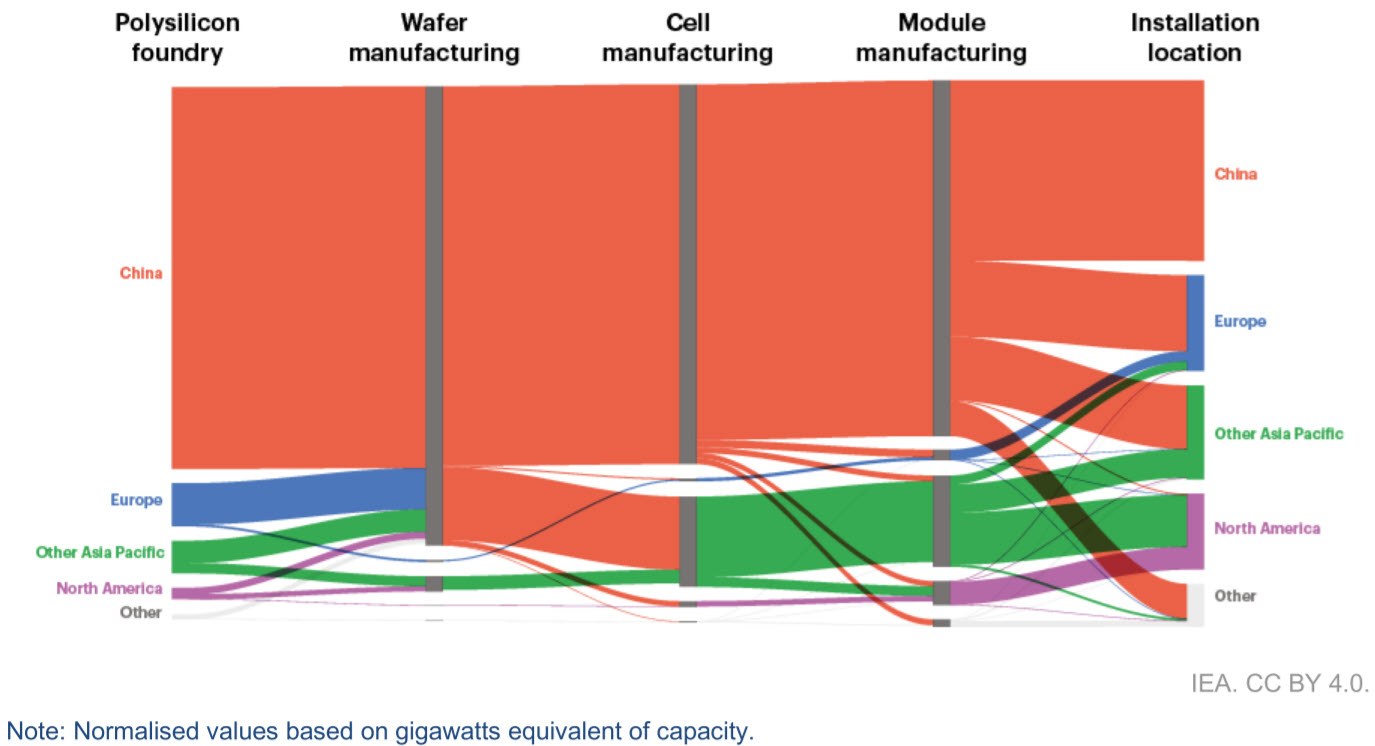
\includegraphics[width=\textwidth]{Images/supply_chain/sankey_diagram_PV_bis.jpg}
    \caption{Flux mondiaux de la chaîne d'approvisionnement du photovoltaïque \cite{iea_energy_2023}}
    \label{fig:PV_sankey}
\end{subfigure}
\hfill
\begin{subfigure}{0.8\textwidth}
    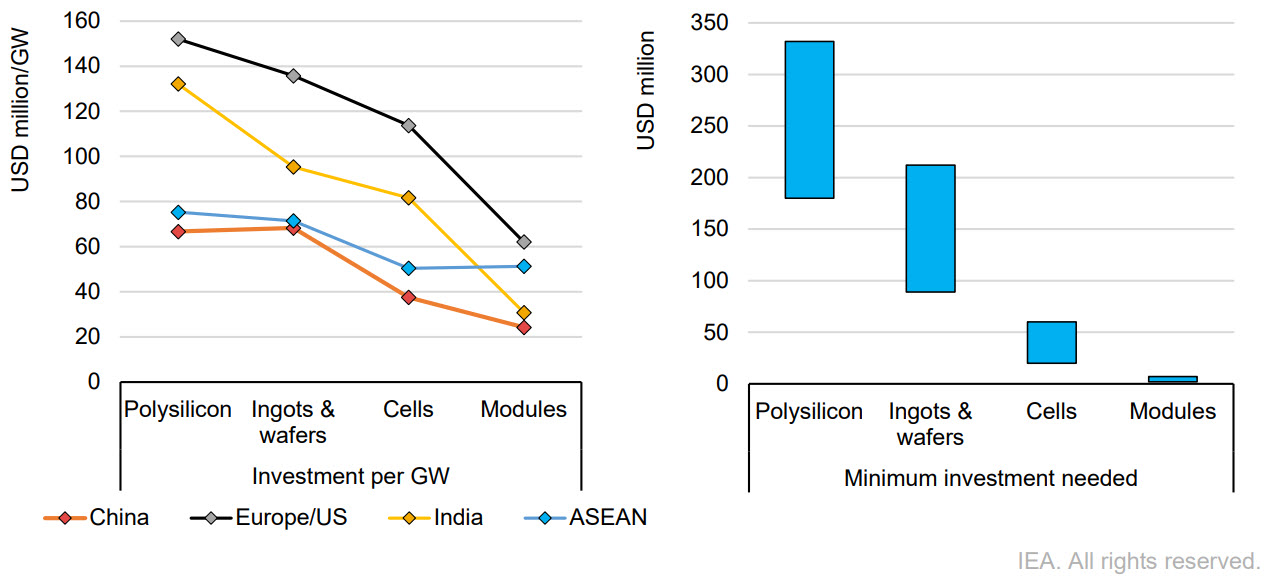
\includegraphics[width=\textwidth]{Images/supply_chain/PV_investment.jpg}
    \caption{Coût d'investissement (gauche) et investissements minimum requis (droite) par étape de la chaîne d'approvisionnement \cite{iea_special_2022}}
    \label{fig:PV_investment}
\end{subfigure}
\begin{subfigure}{0.7\textwidth}
    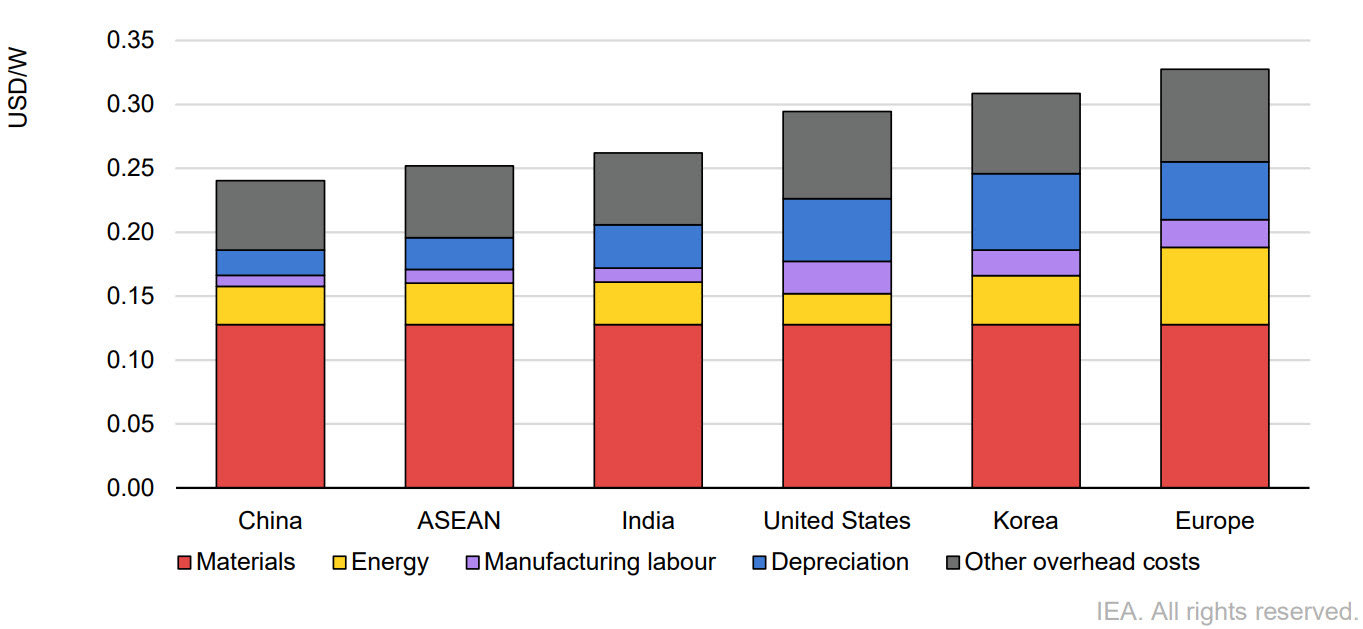
\includegraphics[width=\textwidth]{Images/supply_chain/PV_production_costs.jpg}
    \caption{Coût de production des composants photovoltaïque \cite{iea_special_2022}}
    \label{fig:PV_cost}
\end{subfigure}
  
\caption{Chaîne d'approvisionnement du photovoltaïque}
\label{fig:supply_key_elements_PV}
\end{figure}
\clearpage
\textbf{Eolien}
\smallbreak
Les composants d'une éolienne sont volumineux et lourds, ce qui pénalise une délocalisation de la production. Néanmoins, il est tout à fait possible d'avoir des marchés approvisionnés par une production étrangère. Le marché domestique des Etats-Unis est approvisionné à 75\% par des pales d'éoliennes étrangères (\cite{iea_energy_2023}). La Chine occupe une place importante dans les chaînes d'approvisionnement et représente plus de la moitié des exports de composants éolien (voir figure \ref{fig:wind_sankey}, volume d'exportation en US\$).
\smallbreak
La dépendance envers la Chine dans la filière éolienne est assez modérée. Cependant, il est possible que la Chine produise les composants d'éolienne à des coûts encore plus compétitifs. Le transport de ces éléments étant économiquement viable, il est possible que l'industrie chinoise s'impose sur l'ensemble des marchés mondiaux. Cela aurait pour conséquence de mettre ces marchés dans une situation équivalente aux marchés du photovoltaïque en matière de dépendance envers la Chine.
\begin{figure}[!h]
    \centering
    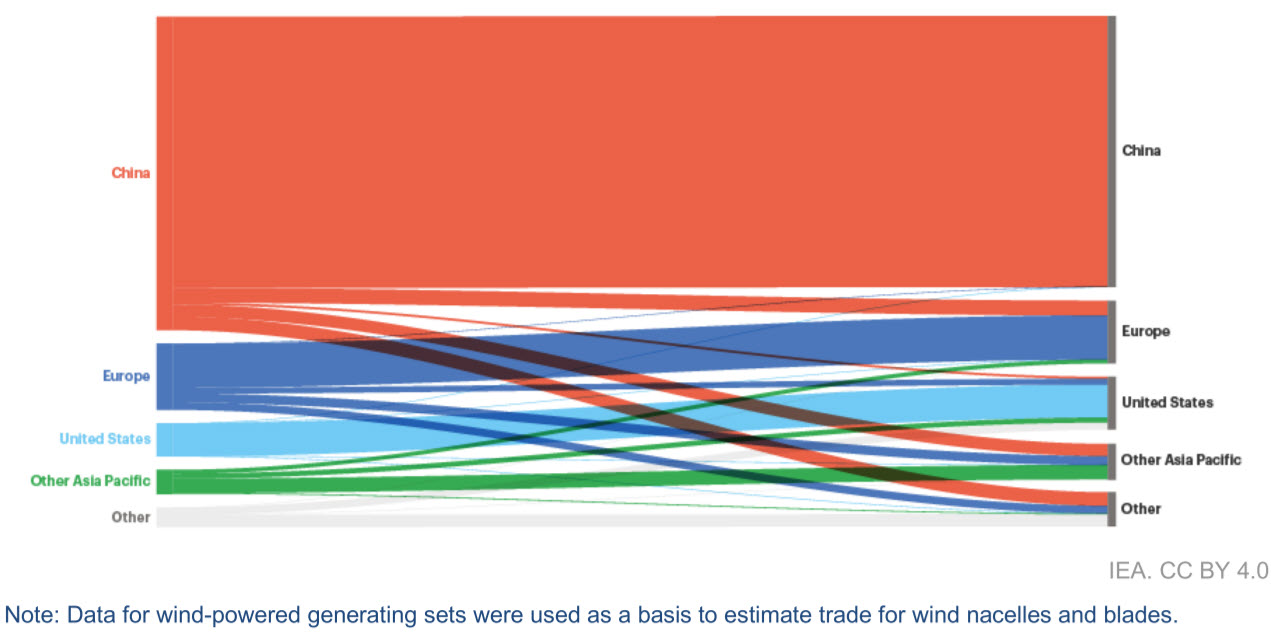
\includegraphics[width=0.8\textwidth]{Images/supply_chain/sankey_diagram_wind.jpg}
    \caption{Flux d'échanges de composants d'éolien (nacelles et pales) en US\$ (\cite{iea_energy_2023})}
    \label{fig:wind_sankey}
\end{figure}
~\\
\textbf{Véhicules électriques}
\smallbreak
Le marché des véhicules électriques est en pleine explosion en partie grâce aux politiques publiques. La Chine occupe une double place dans le marché mondial des véhicules électriques. L'industrie chinoise est la première industrie productrice et exportatrice de batteries pour véhicules électriques et de véhicules électriques (voir figure \ref{fig:EV_sankey}). Le marché chinois du véhicules électriques est quant à lui le plus important dans le monde (en terme de nombre de véhicules vendus).\smallbreak
La production américaine de véhicules électriques repose nettement moins sur les batteries chinoises que la production européenne. Cet écart s'explique en grande partie par des actions publiques américaines pour favoriser les batteries produites localement dès 2009, tandis que l'Union européenne a mis en place une stratégie industrielle sur les batteries en 2017.\smallbreak
L'industrie automobile est souvent un secteur très important de l'économie des pays européens. La décarbonation conduit cette industrie exclusivement vers la production de véhicules électriques dépendants d'un approvisionnement en batterie. Cet approvisionnement en batterie vient actuellement à 15\% de Chine et cette part pourrait augmenter si les capacités de production européennes de batteries n'augmentent pas aussi vite que le marché. Cette situation permet à la Chine d'affecter directement un secteur industriel très important pour l'économie européenne.\smallbreak
Grâce à des coûts de production faibles et à un marché important, la Chine attire les constructeurs de véhicules électriques étrangers. La majeure partie des véhicules électriques importés de Chine sont de constructeurs européens ou américains (voir figure \ref{fig:EV_Europe}).
\begin{figure}[!h]
\centering
\begin{subfigure}{0.8\textwidth}
    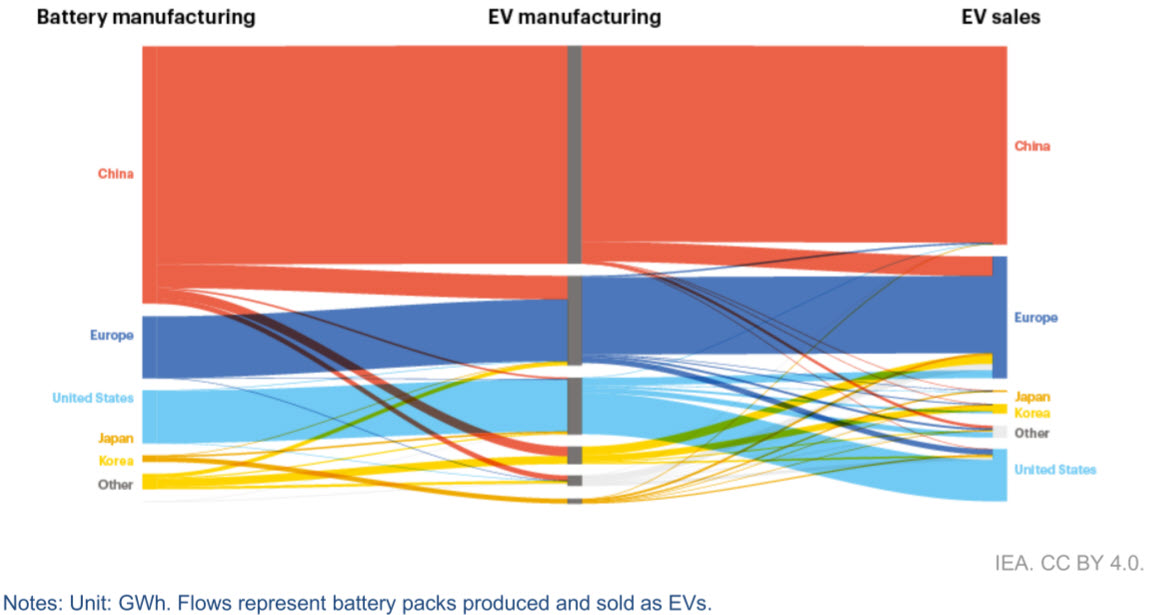
\includegraphics[width=\textwidth]{Images/supply_chain/sankey_diagram_EV.jpg}
    \caption{Flux mondiaux de la chaîne d'approvisionnement des véhicules électriques}
    \label{fig:EV_sankey}
\end{subfigure}
\hfill
\begin{subfigure}{0.8\textwidth}
    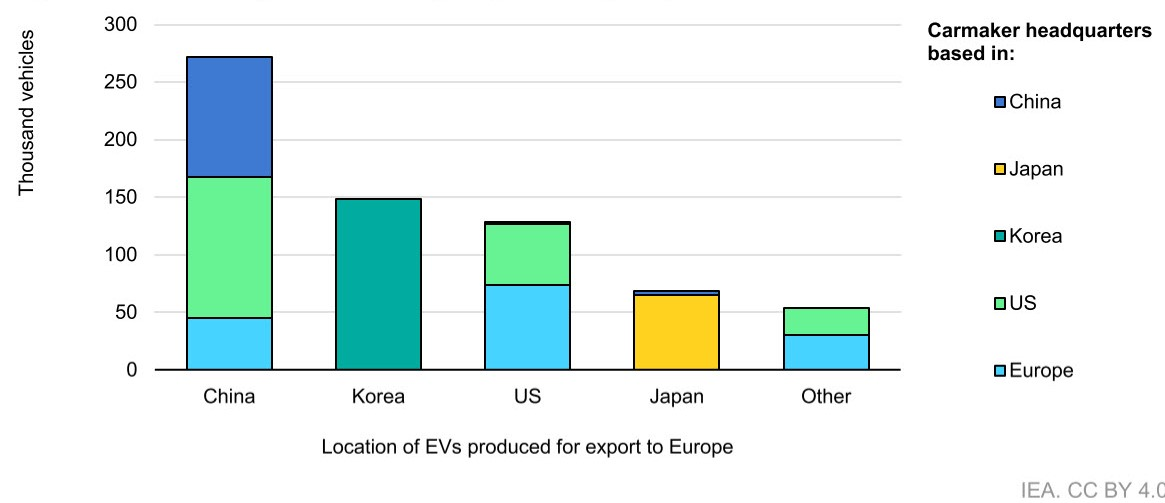
\includegraphics[width=\textwidth]{Images/supply_chain/Europe_EV_imports_bis.jpg}
    \caption{Répartition des importations de véhicules électriques en Europe par pays et par nationalité de fabricant}
    \label{fig:EV_Europe}
\end{subfigure}

\caption{Chaîne d'approvisionnement des véhicules électriques (\cite{iea_energy_2023})}
\label{fig:supply_key_elements_EV}
\end{figure}
\clearpage